%%to compile without ps: latex2pdf file.tex
%%with ps: latex file.tex; dcips file.dvi; ps2pdf file.ps

\documentclass[]{beamer}
%%% BEGIN PREAMBLE
%\mode<presentation>
\usepackage{graphicx}
\usepackage[round]{natbib}
\usepackage{movie15} 
\usepackage{hyperref}
\usepackage{mathtools}
\usepackage{amsmath}
\usepackage{amssymb}

%%
%% Generated by Rodrigo Platte, Arizona State University, May 18 2007 %%
%% Edit this file to change how your presentation looks!
%%
%% For more information, please read the manual: beameruserguide.pdf
%%	 

% Select a theme
%%%%%%%%%%%%%%%%%%%%%%%%%%%
% \usetheme{Frankfurt}
% \usetheme{Singapore}
 %   \usetheme{Madrid}
% \usetheme{Dresden}
%\usetheme{Berlin}
% \usetheme{Boadilla}
 %  \usetheme{Antibes}
 %  \usetheme{Berkeley}
  \usetheme{shadow}
  %\usetheme{default}
%%%%%%%%%%%%%%%%%%%%%%%%%%%

% Select a color theme
%%%%%%%%%%%%%%%%%%%%%%%%%%%
 % \usecolortheme{seagull}
  %\usecolortheme{beetle}
 % \usecolortheme{crane}
  %\usecolortheme{default}
  % \usecolortheme[rgb={.4,0,0}]{structure} % Red colors
  %  \usecolortheme[rgb={.2,0,0}]{structure} % Dark Red colors
 % \usecolortheme[rgb={.6,.5,.2}]{structure} % Yellow/Green colors
%\usecolortheme[rgb={0,.5,.2}]{structure} % Green colors
\usecolortheme[rgb={.5,.1,.5}]{structure} %navy
%%%%%%%%%%%%%%%%%%%%%%%%%%%
  
 % Select a font theme
 %%%%%%%%%%%%%%%%%%%%%%%%%%
   %  \usefonttheme{structurebold}
   %  \usefonttheme{structuresmallcapsserif}
   % \usefonttheme{structureitalicserif}
    %  \usefonttheme{serif}
 %%%%%%%%%%%%%%%%%%%%%%%%%%
% select an inner theme
%\userinnertheme{default}


 % Select a background color  
 %%%%%%%%%%%%%%%%%%%%%%%%%%%%%%
   %\setbeamertemplate{background canvas}[vertical shading][bottom=white,top=gray!30]
  %  \setbeamertemplate{background canvas}[vertical shading][bottom=white,top=red!10!black!30]
   %\setbeamertemplate{background canvas}[vertical shading][bottom=white,top=green!20!black!30]
   % \setbeamertemplate{background canvas}[vertical shading][bottom=white,top=white]
%%%%%%%%%%%%%%%%%%%%%%%%%%%%%%%

% Select a color for math text
%%%%%%%%%%%%%%%%%%%%%%%%%%%%%%% 
% \setbeamercolor{math text}{fg=red!80!black}
%%%%%%%%%%%%%%%%%%%%%%%%%%%%%%%


% This command suppresses the navigation symbols at footline
% comment the command below if you  want navigation symbols 
%\setbeamertemplate{navigation symbols}{}

% Set the size of the font in frame title
\setbeamerfont{frametitle}{size=\normalsize}

%\useoutertheme{sidebar}

% This command will generate a gray footline with the ASU logo in
% each frame
%  \useoutertheme{mathASUlogo}



\bibliographystyle{plainnat}

\definecolor{lightblue}{rgb}{0.8,0.8,1.0}
\definecolor{lightgreen}{rgb}{0.4,1.0,0.4}
\definecolor{purple}{rgb}{0.5,0.1,0.5}
\setbeamercolor{boxcolor}{fg=white,bg=purple}
\DeclareGraphicsExtensions{.jpg, .png}
\title{Kinematics of filaments and its role in star formation}
\author[Britta Hansen]{\bf Britta Hansen}
%\date{April 26, 2013} % delete this line to display the current date

\setbeamertemplate{footline}{\hfill\insertframenumber/\inserttotalframenumber}
\newcommand{\vecnorm}[1]{\left|\left|#1\right|\right|}
%%% BEGIN DOCUMENT
\begin{document}

% create title slide
\begin{frame}
\titlepage
\end{frame}

%Slide 0
\begin{frame}
\frametitle{Filaments}
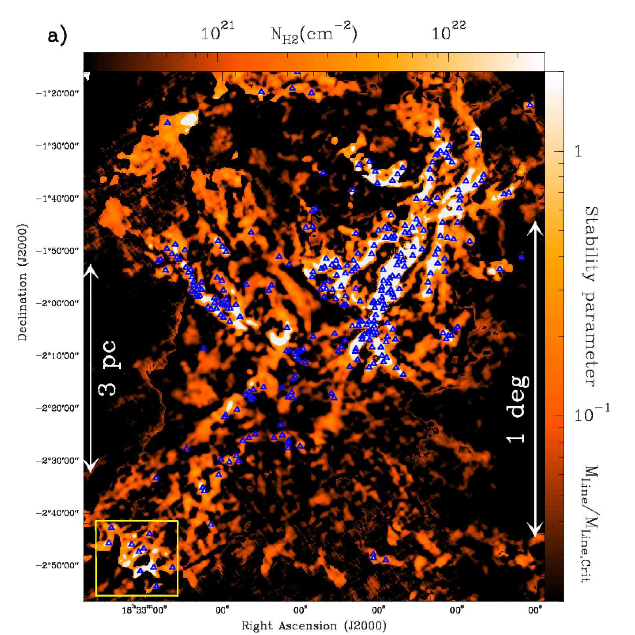
\includegraphics[scale=0.3,natwidth=635,natheight=635]{Aquila} \\ {\centering{ \tiny 	Fig. 6a from \citep{and13}: Column density map from Herschel data of the Aquila star forming region. Blue triangles are thought to be bound prestellar cores.}}
%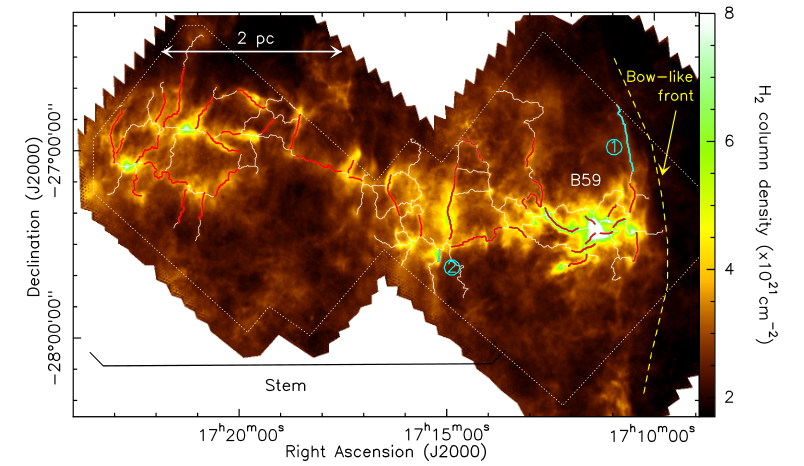
\includegraphics[scale=0.4,natwidth=867,natheight=583]{Pipe_Nebula} \\ {\centering{ \tiny 	Fig. 1 from \citep{per12}: Column density map from Herschel data of the Pipe Nebula. Red lines are filaments traced using an algorithm called DisPerSE.}}
\end{frame}

%Slide 1
\renewcommand*{\thefootnote}{\alph{footnote}}
\begin{frame}
\frametitle{Properties of filaments}
\begin{itemize}
\item Peak column densities $\sim$5x$10^{22}$cm$^{-2}$ %\footnote{\tiny \cite{jml12} \cite{and10}}
\item Width $\sim$0.1pc %\footnote{\tiny \cite{and10} \cite{fm12} \cite{pal13}}
\item Length $\sim$3pc %\footnote{\tiny \cite{and10} \cite{planck33}}
\item Velocity dispersions between $0.2kms^{-1}$ and $10kms^{-1}$ %\footnote{\tiny \cite{arz13}}
\item Magnetic field strength $\simeq15\mu G$ \footnote{\tiny References:\\ \cite{cha11}, \cite{arz13}, \cite{planck33},\\ \cite{and10}, \cite{jml12}}
\item Critical mass per unit length $\sim19M_{\odot}pc^{-1}$
\end{itemize}
\smallskip
\smallskip
\end{frame}

%Slide 2
\begin{frame}
 Critical mass per unit length\\
\begin{align*}
\ell&= \int_0^\infty 2\pi r \rho(r) dr\ \ = \frac{2c_s^2}{G} 
\end{align*} \bigskip \vfil \bigskip \bigskip \bigskip \bigskip \bigskip{ \tiny \cite{im92}, \cite{ost64}}
\end{frame}

%Slide 3
\begin{frame}
\frametitle{Density profiles} %Be sure to draw it and explain all terms
An typical density profile:
\begin{align*}
\rho(r) &= \rho_{max} \left(\sqrt{1 + \left(\frac{r}{H_o}\right)^2}\right)^{-\eta}
\end{align*} $\eta = 4$ for an Ostriker profile.\\ $\eta$ is a free parameter for a Plummer profile.\\
%\begin{align*}
%\rho(r) = \rho_{max}\left(\sqrt{1 + \left(\frac{r}{H_o}\right)^2}\right)^{-\eta}
%\end{align*}
$H_o =\frac{2c_s^2}{\pi G \rho_{max}}$
\end{frame}

%Slide 4
\begin{frame}%mention that discs are about 5 OOM
\frametitle{Filaments and prestellar cores}
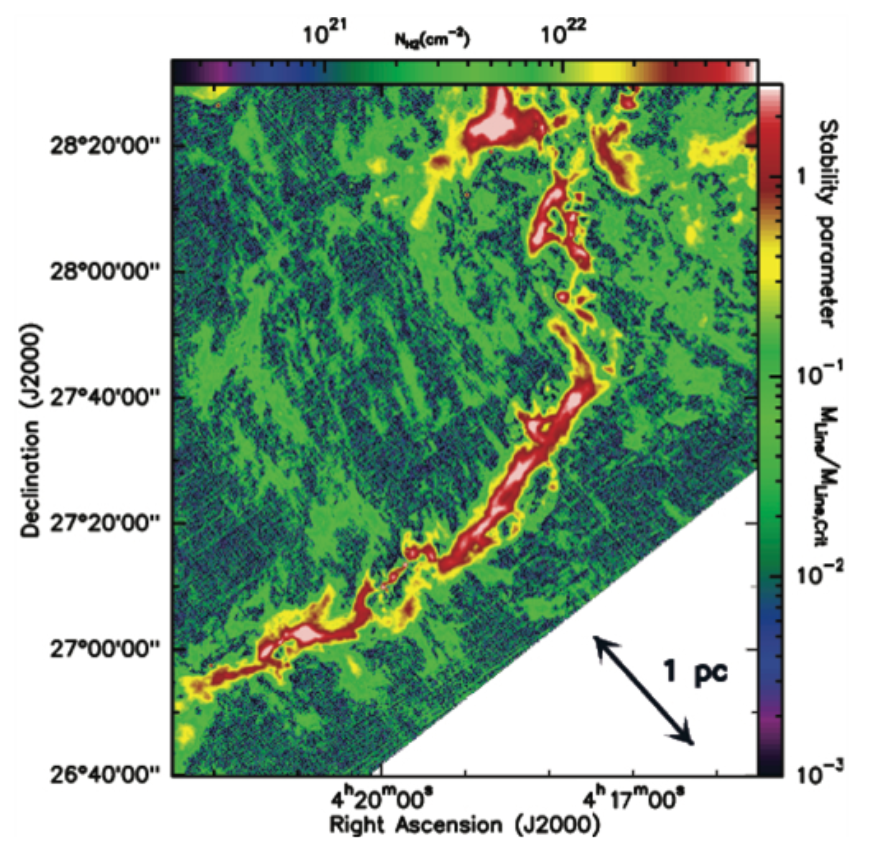
\includegraphics[scale=0.21,natwidth=869,natheight=848]{Taurus_B211} \\ {\centering{ \tiny 	Fig. 2 from \cite{pal13}: Column density map from Herschel data of the filaments B211 and L1495 in Taurus.}}
\end{frame}

%Slide 6
\begin{frame}
\frametitle{Polarization}
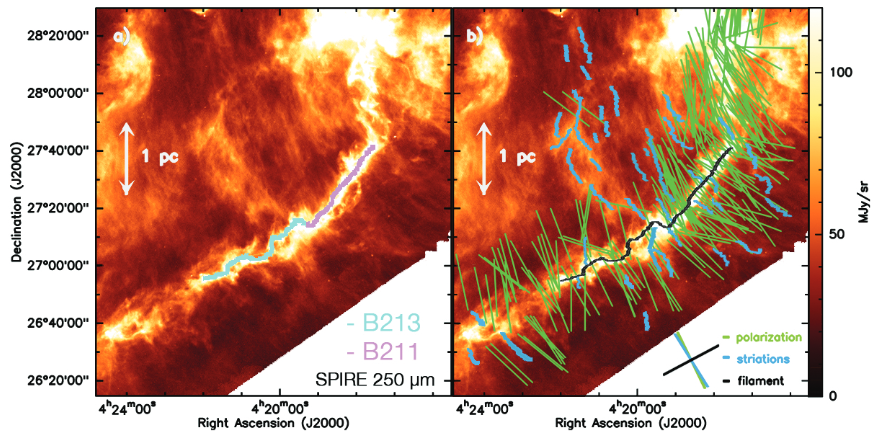
\includegraphics[scale=0.35,natwidth=898,natheight=567]{Herschel_Taurus_B211}\\ {\centering{ \tiny 	Fig. 3 from \cite{pal13}: The filaments B211/B213/L1495 in the TMC, as seen by Herschel.}}
\end{frame}

%Slide 7
\begin{frame}
\frametitle{Research questions}
\begin{itemize}
\item Are filaments really supercritical and collapsing?
\item Which properties of filaments affect star formation?
\item Do striations feed filaments?
\item How are filaments formed?
\end{itemize}
\end{frame}

%Slide 8
\begin{frame}
\frametitle{The code}
RAMSES: AMR, Fortran90, particle data, 3D
\end{frame}

%Slide 9
\begin{frame}
\frametitle{Simulation methodology}
A possible dimensionless parameter of interest:\\
the mass per unit length in units of the critical mass per unit length
\begin{align*}
\eta &=\frac{\rho_{max}\pi R_f^2}{\ell}
\end{align*} Will tell us how magnetic fields and turbulence affect the criticality of the filament.
\end{frame}

%Slide 10
\begin{frame}
\frametitle{Simulation sequence: a single filament}
\begin{enumerate}
\item Static and isothermal
\item Vary density profile
\item Add turbulence
\item Add a magnetic field
\end{enumerate}
\end{frame}

%Slide 11
\begin{frame}
\frametitle{Simulation sequence: a cluster}
\begin{enumerate}
\item Vary the number of filaments
\item Change the mass accretion rates 
\item Add more turbulence to the filaments
\item Add a global magnetic field
\end{enumerate}
\end{frame}

%Slide 12
\begin{frame}
\center Thank you
\end{frame}

%Slide 12
\begin{frame}
\frametitle{Planck results}
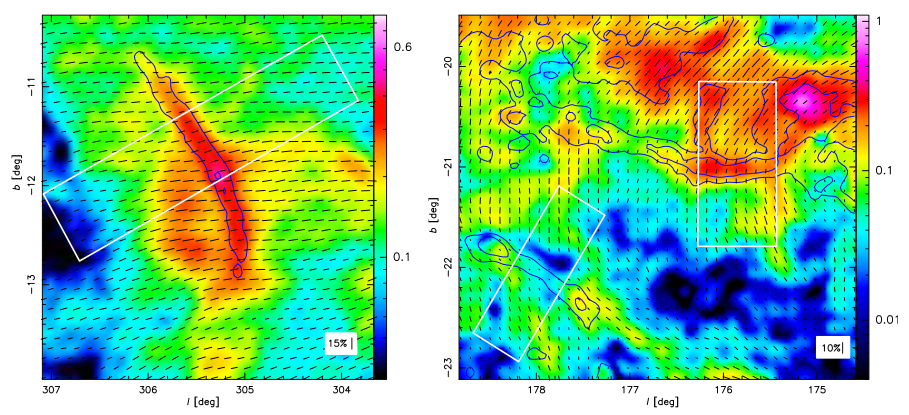
\includegraphics[scale=0.35,natwidth=909,natheight=415]{Planck_polarization}\\ {\centering{ \tiny 	Fig. 10 from \cite{planck33}: Polarization data in the Musca filament (left) and Taurus cloud (right). Emission is in MJy sr$^{-1}$}}
\end{frame}

%Slide 13
\begin{frame}
\frametitle{Planck results 2}
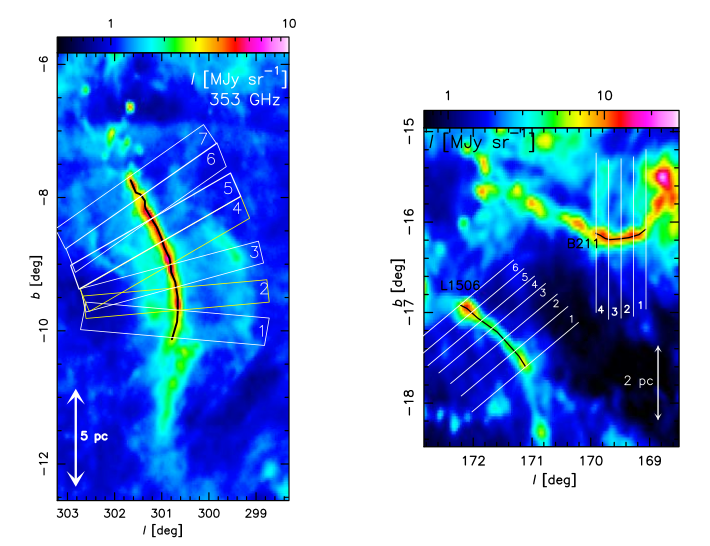
\includegraphics[scale=0.35,natwidth=750,natheight=415]{Stokes_parameters}\\ {\centering{ \tiny 	Figs. 1 and 4 from \cite{planck33}: I band Stokes parameters in the Musca filament (left) and Taurus cloud (right). Emission is in MJy sr$^{-1}$}}
\end{frame}





\bibliography{bibliography}

\end{document}
